\documentclass[conference]{IEEEtran}
\IEEEoverridecommandlockouts
\usepackage{cite}
\usepackage{amsmath,amssymb}
\usepackage{graphicx}
\usepackage{booktabs}
\usepackage{array}
\usepackage{url}
\Urlmuskip=0mu plus 1mu
\usepackage{placeins}
\usepackage[T1]{fontenc}
\usepackage{newtxtext,newtxmath}
\usepackage{textcomp}
\newcommand{\NTradingDays}{3,161}
\newcommand{\DataStart}{2014-01-01}
\newcommand{\DataEnd}{2026-10-09}
\newcommand{\NEquityRowsM}{5.84}
\newcommand{\NEquityRows}{5,836,673}
\newcommand{\NSymbols}{3,748}
\newcommand{\NFOUnderlyings}{354}
\newcommand{\FOPerDayMin}{134}
\newcommand{\FOPerDayMax}{227}
\newcommand{\NStaleFiles}{92}
\newcommand{\NDelivOverlapDates}{12}
\newcommand{\NDelivOverlapMismatch}{0}
\newcommand{\NFOOverlapDays}{5}
\newcommand{\NAdjust}{1,442}
\newcommand{\NAdjustNSE}{841}
\newcommand{\NAdjustGap}{468}
\newcommand{\NAdjustDemerger}{133}
\newcommand{\NGOneChecks}{57}
\newcommand{\GOneMaxDiff}{0}
\newcommand{\NFeatures}{80}
\newcommand{\NBroadTrain}{2,102}
\newcommand{\NBroadVal}{978}
\newcommand{\NBroadTest}{1,796}
\newcommand{\NBroadTotal}{4,876}
\newcommand{\SuccBroad}{0.262}
\newcommand{\NAllTrain}{5,075}
\newcommand{\NAllVal}{1,979}
\newcommand{\NAllTest}{4,273}
\newcommand{\NAllTotal}{11,327}
\newcommand{\SuccAll}{0.249}
\newcommand{\NStrictTrain}{38}
\newcommand{\NStrictVal}{15}
\newcommand{\NStrictTest}{29}
\newcommand{\NStrictTotal}{82}
\newcommand{\SuccStrict}{0.241}
\newcommand{\TvHOneExp}{27.3}
\newcommand{\TvHOneRest}{26.2}
\newcommand{\TvHOneDiff}{+1.0}
\newcommand{\TvHOneP}{0.513}
\newcommand{\TvHOneQ}{0.94}
\newcommand{\TvHTwoExp}{26.7}
\newcommand{\TvHTwoRest}{26.8}
\newcommand{\TvHTwoP}{0.936}
\newcommand{\TvHThreeExp}{1.03}
\newcommand{\TvHThreeRest}{1.07}
\newcommand{\TvHThreeP}{0.801}
\newcommand{\ValAUCxgb}{0.492}
\newcommand{\ValAUCrf}{0.487}
\newcommand{\ValAUClogit}{0.528}
\newcommand{\ValAUCcomp}{0.506}
\newcommand{\XgbTrees}{14}
\newcommand{\XgbDepth}{2}
\newcommand{\HOneExp}{24.8}
\newcommand{\HOneRest}{24.9}
\newcommand{\HOneDiff}{\ensuremath{-}0.04}
\newcommand{\HOneP}{0.987}
\newcommand{\HOneQ}{0.987}
\newcommand{\HTwoExp}{23.5}
\newcommand{\HTwoRest}{26.3}
\newcommand{\HTwoDiff}{\ensuremath{-}2.81}
\newcommand{\HTwoP}{0.171}
\newcommand{\HTwoQ}{0.286}
\newcommand{\HThreeExp}{1.01}
\newcommand{\HThreeRest}{0.88}
\newcommand{\HThreeP}{0.384}
\newcommand{\HThreeQ}{0.480}
\newcommand{\AUCxgb}{0.460}
\newcommand{\AUCrf}{0.466}
\newcommand{\AUClogit}{0.468}
\newcommand{\AUCcomp}{0.526}
\newcommand{\HFourDiff}{\ensuremath{-}0.066}
\newcommand{\HFourSE}{0.023}
\newcommand{\HFourP}{0.005}
\newcommand{\HFourQ}{0.024}
\newcommand{\TopMLPrec}{22.4}
\newcommand{\TopCompPrec}{31.0}
\newcommand{\TopMLN}{165}
\newcommand{\TopP}{0.108}
\newcommand{\TopSpread}{\ensuremath{-}0.26}
\newcommand{\TopSpreadLo}{\ensuremath{-}1.29}
\newcommand{\TopSpreadHi}{+0.64}
\newcommand{\BrierRaw}{0.250}
\newcommand{\BrierCal}{0.195}
\newcommand{\WFAUC}{0.502}
\newcommand{\WFMonths}{46}
\newcommand{\NPHTwoDiff}{\ensuremath{-}5.65}
\newcommand{\NPHTwoP}{0.026}
\newcommand{\NPHTwoQ}{0.128}
\newcommand{\NPHFourDiff}{\ensuremath{-}0.039}
\newcommand{\NPHFourP}{0.141}
\newcommand{\BHm}{5}
\newcommand{\BaseRateTest}{0.248}
\newcommand{\TTwoDiff}{+0.8}
\newcommand{\TTwoP}{0.586}
\newcommand{\PowRuleN}{144}
\newcommand{\PowRuleDiff}{\ensuremath{-}0.2}
\newcommand{\PowRuleP}{0.978}
\newcommand{\LadBaseN}{159,972}
\newcommand{\LadBase}{26.7}
\newcommand{\LadAll}{24.9}
\newcommand{\LadAllDiff}{\ensuremath{-}1.9}
\newcommand{\LadAllP}{0.005}
\newcommand{\LadBroad}{24.8}
\newcommand{\LadComp}{41.4}
\newcommand{\LadCompN}{29}
\newcommand{\CagrAll}{\ensuremath{-}26.8}
\newcommand{\TradesAll}{2,736}
\newcommand{\MaxDDAll}{\ensuremath{-}68.6}
\newcommand{\CagrBroad}{\ensuremath{-}12.6}
\newcommand{\TradesBroad}{1,599}
\newcommand{\MaxDDBroad}{\ensuremath{-}39.2}
\newcommand{\CagrComp}{+6.0}
\newcommand{\TradesComp}{29}
\newcommand{\MaxDDComp}{\ensuremath{-}1.0}
\newcommand{\CagrML}{+4.3}
\newcommand{\TradesML}{157}
\newcommand{\MaxDDML}{\ensuremath{-}2.3}
\newcommand{\CagrNifty}{+9.7}
\newcommand{\SPAp}{0.77}
\newcommand{\CashRate}{6}
\newcommand{\SharpeComp}{\ensuremath{-}0.01}
\newcommand{\SharpeML}{\ensuremath{-}0.85}
\newcommand{\MaxPositions}{20}
\newcommand{\RCp}{0.89}
\newcommand{\DSRtrials}{89}
\newcommand{\TrialsBefore}{67}
\newcommand{\TrialsTestRun}{22}
\newcommand{\TrialsThroughPSix}{89}
\newcommand{\PreregCommit}{15103f1}
\newcommand{\PreregTime}{08:54}
\newcommand{\LockHead}{ea49def}
\newcommand{\LockStart}{09:23}
\newcommand{\LockCommit}{359bcc7}
\newcommand{\LockCommitTime}{09:30}
\newcommand{\TostHOneLo}{\ensuremath{-}3.7}
\newcommand{\TostHOneHi}{+3.6}
\newcommand{\TostHOneP}{0.19}
\newcommand{\TostHTwoLo}{\ensuremath{-}6.2}
\newcommand{\TostHTwoHi}{+0.6}
\newcommand{\TostHTwoP}{0.65}
\newcommand{\TostNPHOneLo}{\ensuremath{-}1.9}
\newcommand{\TostNPHOneHi}{+7.2}
\newcommand{\TostNPHOneP}{0.59}
\newcommand{\TostNPHTwoLo}{\ensuremath{-}9.8}
\newcommand{\TostNPHTwoHi}{\ensuremath{-}1.5}
\newcommand{\TostNPHTwoP}{0.93}
\newcommand{\MDEHOne}{6.26}
\newcommand{\MDEHTwo}{5.71}
\newcommand{\ExpN}{47}
\newcommand{\ExpRemoved}{331}
\newcommand{\ExpDiff}{\ensuremath{-}1.4}
\newcommand{\ExpP}{0.572}
\newcommand{\ExpPMin}{0.516}
\newcommand{\PSIpcr}{0.55}
\newcommand{\PSIclient}{0.31}
\newcommand{\PSInModerate}{7}
\newcommand{\PSInLarge}{2}
\newcommand{\BrierConstVal}{0.188}
\newcommand{\BrierConstTest}{0.187}
\newcommand{\IncompleteBroad}{4}
\newcommand{\GapEvents}{165}
\newcommand{\GapTrades}{157}
\newcommand{\GapSlotsFull}{8}
\newcommand{\RoundTrip}{0.58}
\newcommand{\RTLarge}{0.45}
\newcommand{\RTSmall}{0.75}
\newcommand{\AvgWin}{+4.74}
\newcommand{\AvgLoss}{\ensuremath{-}1.85}
\newcommand{\WinLossSpread}{6.59}
\newcommand{\BreakEven}{8.8}
\newcommand{\BEHOneDiff}{\ensuremath{-}0.0}
\newcommand{\BEHOneLo}{\ensuremath{-}4.4}
\newcommand{\BEHOneHi}{+4.3}
\newcommand{\BEHOneBLo}{\ensuremath{-}5.3}
\newcommand{\BEHOneBHi}{+4.7}
\newcommand{\BEHOneN}{1265}
\newcommand{\BEHTwoDiff}{\ensuremath{-}2.8}
\newcommand{\BEHTwoLo}{\ensuremath{-}6.8}
\newcommand{\BEHTwoHi}{+1.2}
\newcommand{\BEHTwoBLo}{\ensuremath{-}8.3}
\newcommand{\BEHTwoBHi}{+2.1}
\newcommand{\BEHTwoN}{924}
\newcommand{\BENPHOneDiff}{+2.6}
\newcommand{\BENPHOneLo}{\ensuremath{-}2.8}
\newcommand{\BENPHOneHi}{+8.1}
\newcommand{\BENPHOneBLo}{\ensuremath{-}2.8}
\newcommand{\BENPHOneBHi}{+7.9}
\newcommand{\BENPHOneN}{899}
\newcommand{\BENPHTwoDiff}{\ensuremath{-}5.6}
\newcommand{\BENPHTwoLo}{\ensuremath{-}10.6}
\newcommand{\BENPHTwoHi}{\ensuremath{-}0.7}
\newcommand{\BENPHTwoBLo}{\ensuremath{-}12.3}
\newcommand{\BENPHTwoBHi}{+0.7}
\newcommand{\BENPHTwoN}{617}
\newcommand{\BEMLDiff}{\ensuremath{-}2.7}
\newcommand{\BEMLLo}{\ensuremath{-}9.4}
\newcommand{\BEMLHi}{+4.1}
\newcommand{\BEMLBLo}{\ensuremath{-}13.8}
\newcommand{\BEMLBHi}{+7.3}
\newcommand{\BEMLN}{165}
\newcommand{\BECompTopDiff}{+7.0}
\newcommand{\BECompTopLo}{+0.6}
\newcommand{\BECompTopHi}{+13.4}
\newcommand{\BECompTopBLo}{+0.8}
\newcommand{\BECompTopBHi}{+15.0}
\newcommand{\BECompTopN}{226}
\newcommand{\BECompRuleDiff}{+16.8}
\newcommand{\BECompRuleLo}{\ensuremath{-}1.2}
\newcommand{\BECompRuleHi}{+34.9}
\newcommand{\BECompRuleBLo}{\ensuremath{-}10.0}
\newcommand{\BECompRuleBHi}{+46.3}
\newcommand{\BECompRuleN}{29}
\newcommand{\BEnBelow}{3}
\newcommand{\SpecOneN}{54}
\newcommand{\SpecOnePred}{89}
\newcommand{\SpecOneSig}{15}
\newcommand{\SpecOneSigPct}{28}
\newcommand{\SpecOneOpp}{0}
\newcommand{\SpecOneBH}{3}
\newcommand{\SpecOneMedian}{+2.36}
\newcommand{\SpecOneMax}{5.05}
\newcommand{\SpecOneCIAbove}{4}
\newcommand{\SpecOneFrozen}{\ensuremath{-}0.04}
\newcommand{\SpecOneRank}{49}
\newcommand{\SpecTwoN}{18}
\newcommand{\SpecTwoPred}{94}
\newcommand{\SpecTwoSig}{3}
\newcommand{\SpecTwoSigPct}{17}
\newcommand{\SpecTwoOpp}{0}
\newcommand{\SpecTwoBH}{0}
\newcommand{\SpecTwoMedian}{\ensuremath{-}2.24}
\newcommand{\SpecTwoMax}{4.44}
\newcommand{\SpecTwoCIAbove}{0}
\newcommand{\SpecTwoFrozen}{\ensuremath{-}2.81}
\newcommand{\SpecTwoRank}{6}
\newcommand{\BFOneUni}{17.88}
\newcommand{\BFNPOneUni}{9.31}
\newcommand{\BFOneSkep}{2.27}
\newcommand{\BFNPOneSkep}{1.27}
\newcommand{\BFOneLogDef}{8.41}
\newcommand{\BFNPOneLogDef}{4.49}
\newcommand{\BFOneLogSkep}{2.32}
\newcommand{\BFNPOneLogSkep}{1.43}
\newcommand{\BFTwoUni}{7.65}
\newcommand{\BFNPTwoUni}{1.31}
\newcommand{\BFTwoSkep}{1.05}
\newcommand{\BFNPTwoSkep}{0.23}
\newcommand{\BFTwoLogDef}{3.63}
\newcommand{\BFNPTwoLogDef}{0.67}
\newcommand{\BFTwoLogSkep}{1.13}
\newcommand{\BFNPTwoLogSkep}{0.30}
\newcommand{\EOneBOne}{+0.008}
\newcommand{\EOneBOneLo}{\ensuremath{-}0.237}
\newcommand{\EOneBOneHi}{+0.254}
\newcommand{\EOneBOneP}{0.946}
\newcommand{\EOneBTwo}{\ensuremath{-}0.225}
\newcommand{\EOneBTwoLo}{\ensuremath{-}0.592}
\newcommand{\EOneBTwoHi}{+0.142}
\newcommand{\EOneBTwoP}{0.229}
\newcommand{\EOneBThree}{+0.246}
\newcommand{\EOneBThreeLo}{\ensuremath{-}0.130}
\newcommand{\EOneBThreeHi}{+0.622}
\newcommand{\EOneBThreeP}{0.200}
\newcommand{\ETwoBOne}{\ensuremath{-}0.129}
\newcommand{\ETwoBOneLo}{\ensuremath{-}0.361}
\newcommand{\ETwoBOneHi}{+0.102}
\newcommand{\ETwoBOneP}{0.273}
\newcommand{\ETwoBTwo}{+0.185}
\newcommand{\ETwoBTwoLo}{+0.006}
\newcommand{\ETwoBTwoHi}{+0.364}
\newcommand{\ETwoBTwoP}{0.043}
\newcommand{\ETwoBThree}{\ensuremath{-}0.186}
\newcommand{\ETwoBThreeLo}{\ensuremath{-}0.435}
\newcommand{\ETwoBThreeHi}{+0.063}
\newcommand{\ETwoBThreeP}{0.142}
\newcommand{\EMonthMatches}{exactly}
\newcommand{\FYears}{12}
\newcommand{\FYearsSig}{0}
\newcommand{\FFirstYear}{2015}
\newcommand{\FLastYear}{2026}
\newcommand{\GTieShareLoss}{0.12}
\newcommand{\GTieExplained}{0.1}
\newcommand{\GDayOneBO}{15.0}
\newcommand{\GDayOneNB}{10.3}
\newcommand{\GRangeBO}{1.07}
\newcommand{\GRangeNB}{0.95}
\newcommand{\GGapBO}{0.11}
\newcommand{\GGapNB}{0.05}
\newcommand{\GATRBO}{2.55}
\newcommand{\GATRNB}{2.68}
\newcommand{\GAgree}{100.0}
\newcommand{\placeboDraws}{1,000}
\newcommand{\placeboActual}{\ensuremath{-}0.04}
\newcommand{\placeboMean}{+1.65}
\newcommand{\placeboSD}{1.97}
\newcommand{\placeboP}{0.795}
\newcommand{\placeboPct}{20}
\newcommand{\PSevenActual}{+1.05}
\newcommand{\PSevenDraws}{20}
\newcommand{\PSevenGE}{0}

\ifdefined\XeTeXrevision\setmonofont{texgyrecursor-regular.otf}\fi
\begin{document}

\title{Do Delivery and Futures-Positioning Footprints Predict Breakout Success? A Pre-Registered Test on Survivorship-Free NSE Data}

\author{
\IEEEauthorblockN{Anonymous Authors}
}

\maketitle

\begin{abstract}
Two ``free'' daily tracks that traders in India watch to gauge informed activity in a stock are (1) the
delivery percentage of quantity traded that is settled into investors' accounts and (2) changes in futures
positions. Can these identify successful price breakout events? We recreate a survivorship-free,
corporate-action-adjusted panel from official National Stock Exchange of India (NSE) files (2014-01-01 to
2026-10-09, 3,748 symbols), mark breakouts by triple barriers (2 up average true range, 1 down; 10 days) and
assess four hypotheses that are all in version control before we conduct any confirmatory study. We check the
test set (January 2023 to 2026-10-09) once. No hypotheses are verified. Expanding deliveries affect success in
the test set by \ensuremath{-}0.04 percentage points (pp) ($p=0.987$). Price up, open interest (OI) down is the
right sign (\ensuremath{-}2.81 pp), but does not pass false discovery control ($q=0.286$). A gradient-boosted
model sorts breakouts worse than fixed-weight composite (0.460 vs.\ 0.526 area under the curve). The setup has
power to spot effects of size around 6.26 pp. So lower effects cannot be excluded. 95\% confidence intervals for
the delivery and OI effects in post-hoc analyses of the entire test set are inside the 8.8 pp swing in success
rate needed to pay for one round trip of Indian trading costs. No strategy's post-costs return exceeds the
Nifty~500 index.
\end{abstract}

\begin{IEEEkeywords}
backtest overfitting, breakout, delivery percentage, multiple testing, National Stock Exchange of India, open
interest, pre-registration
\end{IEEEkeywords}

\section{Introduction}
Recent IEEE studies forecast Indian and global stock prices with boosted trees, deep ensembles and
explainable AI \cite{samantaray2026,singh2025,kumar2025,rajagopal2026}. Intraday data have been used to construct indicators of informed trading and ``flow toxicity''
\cite{easley1996,easley2012}. Informed trading theories suggest that more informed traders imprint their
presence on price and order flow \cite{kyle1985,glosten1985}. These theories are only motivation; we don't
measure order flow toxicity. We don't use intraday data. We work with free end-of-day data of National Stock
Exchange of India (NSE). There are two footprints of informed activity that traders can read: 1) delivery
percentage, 2) positioning on futures (i.e., a stock's own open interest (OI), NSE reported market-wide positions
for foreign institutional investors (FIIs), domestic institutional investors (DIIs), proprietary desks, and
clients). It's believed that high delivery with supportive positioning on a breakout is ``real''.

Since published signals are often picked from a large set of trial specifications
\cite{harvey2016,bailey2014pseudo}, we designed the study to credibly provide a negative result
\cite{nosek2018}. Pre-registering 4 hypotheses on BROAD compression breakouts (Section~\ref{sec:method}):
\textbf{H1}: breakouts with a delivery expansion base tend to succeed more often. \textbf{H2}: breakouts with
price increasing while futures OI of the stock decreasing tend to fail more often. \textbf{H3}: breakouts when
FII net selling / DII net buying tends to have better gain/loss ratio. \textbf{H4}: Gradient-boosted tree model
(XGBoost \cite{chen2016}) with the same features is superior to a constant-weight composite in both area under
receiver operating characteristic curve (AUC) and top-decile precision.

Contributions: (i) IMPI: a pipeline to reconstruct a survivorship-free point-in-time (PIT) NSE panel including
pre-2019 delivery data that is not available via the current NSE interface. (ii) Pre-registered study design.
One time test set open. Publicly available timeline. (iii) A confirmatory null result with minimum detectable
effect, and a cost-based interpretation of relevant effect sizes. (iv) Post hoc robustness tests clearly
distinguished, to indicate the range and limits of the null.

\section{Related Work}
\emph{Informed-flow theory.} Gradual insider trading of Kyle to assimilate information \cite{kyle1985}.
Glosten--Milgrom, adverse selection embedded in spread pricing \cite{glosten1985}. PIN (probability of informed
trading) and volume-synchronized PIN (VPIN) for measuring informed trading through trade imbalance
\cite{easley1996,easley2012}. Require trade-level data. We merely adopt the idea of daily footprint of informed
trading.
\emph{Institutional flows in India.} Fast selling of Indian stocks post unexpected tax-policy shock by FII and
historical return chasing \cite{thapa2026}. We cannot access daily flow (at the firm level) of FII. We can use
participant positioning as a market regime here. We have not seen peer-reviewed test of NSE delivery and/or
futures position as predictor of breakout success.
\emph{Machine learning (ML) for stock prediction.} Non-linear models are said to outperform linear (but not
often out-of-firm \cite{lu2024})
\cite{fieberg2023,azevedo2023,farimani2024}. On NSE data, Samantaray et al.\ tune a light gradient boosting
machine (LightGBM) with constricted particle swarm optimization on wavelet bands and add Dow Jones signals to
forecast three NSE indices \cite{samantaray2026}. Wavelet-denoised LSTM--CNN--TCN ensembles \cite{singh2025}
and a stacked XGBoost, LightGBM and SVR model \cite{kumar2025} also report low price errors on the Nifty~50.
These studies forecast index prices; we ask a different question, whether a single breakout succeeds. Now
widespread to use Shapley additive explanations (SHAP) for tree-ensembles \cite{lundberg2020} in ML for finance
\cite{cerneviciene2024,martins2024,yeo2025}. SHAP scores, together with out-of-sample Sharpe ratio and drawdown,
have also been used to screen machine-learned alpha factors on S\&P~500 stocks \cite{rajagopal2026}. Test
XGBoost versus simple rule.
\emph{Multiple testing and backtest overfitting.} Number of test $\rightarrow$ significance threshold should
increase \cite{harvey2016}. Deflated Sharpe ratio (DSR) adjusts for trials and nonnormality
\cite{bailey2014dsr}. We adopt Benjamini--Hochberg (BH) \cite{benjamini1995}. Hansen's test for superior
predictive ability (SPA) \cite{hansen2005}. White's reality check \cite{white2000}. Log each trial.

\section{Data and Method}\label{sec:method}
\begin{figure*}[t]
\centering
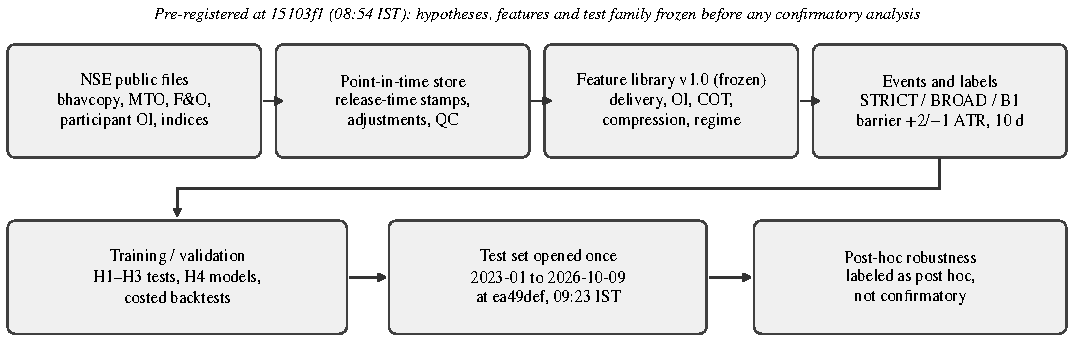
\includegraphics[width=\textwidth]{figs/fig1_pipeline.pdf}
\caption{The IMPI pipeline. Every stage reads only data published by the decision time.}
\label{fig:pipeline}
\end{figure*}

\emph{Data} (Fig.~\ref{fig:pipeline}, Table~\ref{tab:dataset}). NSE data end-of-day data files have 3,161
trading days with 5.84 million daily rows of equities for 3,748 symbols (including delisted stocks). The F\&O
eligible symbols are selected PIT (354 underlyings, 134--227 daily). For delivery before 2019, the delivery file
is reconstructed from legacy equity file and security level delivery position file (MTO), which matches the
modern file (0 mismatches on 12 overlap dates). 1,442 split / bonus / demerger price, volume and OI adjustments
are made. QC of files is automated.

\emph{Universe/Lookahead:} Tier~1: F\&O stocks (on that day, except for ban-list days) excluding result
announcement periods, prices less than Rs~20 and less history. Split: Train (June 2015--2020) Val (2021--2022),
Test (Jan 2023 to 2026-10-09). Purge labels crossing split boundaries. Features on day $T$ use data only until
23:59 Indian Standard Time (IST) on $T$. Entries at $T+1$ Open. No historical change when recomputing features
on 57 truncated copies.

\emph{Events and label.} STRICT events are an algorithmic pattern of vol contraction (VCP)
\cite{minervini2013}. BROAD events are closes above previous 20 days high after compression (bollinger-width
percentile $<$30 for 5 days out of last 10); B1 = all closes at 20-day highs (Table~\ref{tab:events}). At entry
$E$ at $T+1$ open, $A$ = 14 day average true range (ATR), $y=1$ if $E+2A$ was reached before $E-A$ within 10
days, else $y=0$ \cite{lopezdeprado2018}. Day touching both barriers is a loss. 4 BROAD events with imperfect
windows are excluded.

\begin{table}[t]
\centering
\caption{Dataset summary (official NSE files)}
\label{tab:dataset}
\footnotesize
\setlength{\tabcolsep}{4pt}
\begin{tabular}{@{}>{\raggedright\arraybackslash}p{3.7cm}>{\raggedright\arraybackslash}p{4.4cm}@{}}
\toprule
\textbf{Item} & \textbf{Value} \\
\midrule
Period & 2014-01-01 to 2026-10-09 \\
Trading days & 3,161 \\
Daily equity rows & 5,836,673 \\
Symbols (incl.\ delisted) & 3,748 \\
Futures and options (F\&O) underlyings & 354 over time; 134--227 per day \\
Delivery rebuild vs.\ modern file & 0 mismatches on 12 overlap dates \\
F\&O old vs.\ new file format & 0 mismatches on 5 overlap days \\
Stale files rejected & 92 \\
Duplicate symbol-date rows & 0 \\
Delivery coverage (worst year) & 99.33\% \\
Corporate-action adjustments & 1,442 \\
\bottomrule
\end{tabular}
\end{table}
\begin{table}[t]
\centering
\caption{Tier-1 eligible events by split (frozen before registration)}
\label{tab:events}
\footnotesize
\setlength{\tabcolsep}{4pt}
\begin{tabular}{@{}lrrrrr@{}}
\toprule
\textbf{Event set} & \textbf{Train} & \textbf{Val.} & \textbf{Test} & \textbf{Purged} & \textbf{Success} \\
\midrule
STRICT (VCP) & 38 & 15 & 29 & 1 & 0.241 \\
BROAD & 2,102 & 978 & 1,796 & 131 & 0.262 \\
B1 (20-day highs) & 5,075 & 1,979 & 4,273 & 282 & 0.249 \\
\bottomrule
\end{tabular}
\par\smallskip\parbox{0.98\linewidth}{\scriptsize\raggedright Purged = label window crosses a split boundary or is incomplete. Success = share with label$_{10}=1$ (all splits).}
\end{table}

\emph{Tests/Models.} 80 frozen features. Delivery, volume, illiquidity, compression, VCP, stock OI, COT
(participant positioning) style. Index and stock futures. Basis. Put/call ratio. Regime. Comparison of success
rates. H1, H2 (two-proportion $z$-test; block bootstrap, calendar month). H3: gain/loss ratio. Mean favourable /
mean adverse excursion. Logistic model.
\begin{equation}
\operatorname{logit}\Pr(y=1)=\beta_0+\beta_1 D+\beta_2 P+\beta_3 (D\times P)+\gamma^{\top}x,
\label{eq:logit}
\end{equation}
where $D$ is the exposure and $P$ is another variable (H1: alignment of positioning, H2: delivery
$z$-score), to estimate $\beta_3$ of the interaction, with controls for turnover, volatility, liquidity, sector,
$x$. Family of eight pre-registered tests (H1--H3 for STRICT, BROAD, H4-AUC, H4-top-decile) corrected by BH for
$q=0.10$. Group with less than 30 events doesn't have $p$-value. Isotonically calibrated to validation data:
XGBoost (random forest and logistic regression too) with purged, embargoed 5-fold cross validation tuning.
Comparison with composite by DeLong's test \cite{delong1988}. Trade Rs~10~lakh, at most 20 equal weight
positions with all Indian delivery costs, plus 5--20bp of slippage per side, vs Nifty~500, backtest.

\section{Pre-Registration and Integrity}\label{sec:prereg}
Hypotheses, events, test family and decision rules: version \texttt{15103f1} committed at 08:54 IST 10
October 2026 with frozen features (Table~\ref{tab:timeline}). \emph{Lock:} The single test run began at 09:23
IST on commit \texttt{ea49def} (code and training/validation results) and created the lock file, first
committed \texttt{359bcc7} at 09:30. \emph{Trials:} 67 of the 89 rows in the results log until the test
evaluation occurred before the test run. The test run created 22. The DSR used all 89 (conservative).
\emph{Disclosure:} The entire period was used for data download and corporate-action corrections and QC. The
pre-registration lists for its power calculation event counts and total success rate by split (including test)
but not results by split by any hypothesis exposure. For our pilot study we considered July 2025 until October
2026. For confirmatory results we also show them without that window.

\begin{table}[t]
\centering
\caption{Pre-registration timeline, 10 Oct 2026 (IST, from git and run logs)}
\label{tab:timeline}
\footnotesize
\setlength{\tabcolsep}{4pt}
\begin{tabular}{@{}ll>{\raggedright\arraybackslash}p{5.9cm}@{}}
\toprule
\textbf{Commit} & \textbf{Time} & \textbf{Event} \\
\midrule
\texttt{355cbe0} & 02:16 & Pipeline scaffolding: ingest, PIT store, features, labels \\
\texttt{86ddfd7} & 08:21 & Corporate-action adjustment fixes (full data) \\
\texttt{b5829b2} & 08:40 & Ban-list publication-time fix (look-ahead check) \\
-- & 08:53 & Feature freeze written (features, events, labels) \\
\texttt{15103f1} & 08:54 & Pre-registration (H1--H4, rules, power) and feature freeze \\
-- & 08:54 & First training/validation analysis rows logged \\
\texttt{ea49def} & 09:23 & Training/validation results and model freeze \\
-- & 09:23 & Test run starts: test set opened; lock written (HEAD = ea49def) \\
\texttt{359bcc7} & 09:30 & One-time test evaluation and lock file \\
\texttt{1fc97ae} & 12:01 & First post-hoc work (v2 models, live mode) \\
\bottomrule
\end{tabular}
\par\smallskip\parbox{0.98\linewidth}{\scriptsize\raggedright 67 of the 89 results (rows from log upto test evaluation) were pretest written, the other 22 are test run specific rows. The first time the lockfile was commited was in 359bcc7. The full period was used for data download, adjust fixes, QC (pre pre-registration). Pre registration has e.g. counts for events in test set, and the overall test success rate (power table). But no result per hypothesis exposure.}
\end{table}

\section{Results}
\subsection{Exploratory (Training and Validation)}
Training \& Validation data: BROAD with Delivery Expansion: 27.3\% success rate (vs 26.2\%: +1.0 pp,
$p=0.513$). H2: 26.7\% (vs 26.8\%, $p=0.936$). H3 ratio: 1.03 (vs 1.07, $p=0.801$). XGBoost has a validation AUC
of 0.492 (early stopping: 14 trees, depth of 2). Random forest AUC: 0.487. Logistic model AUC: 0.528. Composite
AUC: 0.506.

\subsection{Confirmatory (Test Set, Run Once, Pre-Registered)}
All STRICT groups have less than 30 events per arm. Thus, $p$ values are suppressed and BH runs over $m=5$
finite $p$ values (Table~\ref{tab:confirm}). None's supported. \textbf{H1:} 24.8\% vs.\ 24.9\%
(\ensuremath{-}0.04 pp, $p=0.987$). \textbf{H2:} 23.5\% vs.\ 26.3\% (\ensuremath{-}2.81 pp, $q=0.286$);
omitting pilot window \ensuremath{-}5.65 pp ($p=0.026$, $q=0.128$). \textbf{H3:} 1.01 vs.\ 0.88 ($p=0.384$).
\textbf{H4:} XGBoost AUC 0.460 vs.\ 0.526 composite (difference \ensuremath{-}0.066, DeLong $p=0.005$,
$q=0.024$), only rejection (the wrong way); forest 0.466; logit 0.468; walk-forward (46 refits) 0.502; Top
decile precision 22.4\% vs.\ 31.0\% ($p=0.108$).

In particular, the model used widespread features of market positioning that changed their distributions.
We find a post hoc population stability index (PSI) of 0.55 for the put--call ratio and 0.31 for client
positioning in index futures, which exceeds the usual cutoff of 0.25. The calibration reduced the Brier score
\cite{brier1950} from 0.250 to 0.195, which is still worse than a constant forecast at validation base rate
(0.188).

\emph{Power.} The power of the design is 80\% for $\alpha=0.05$ with 6.26 pp (H1), 5.71 pp (H2). Smaller
effects are possible. No equivalence is shown within $\pm$2 pp (post-hoc two one-sided tests (TOST)
\cite{lakens2017}: 90\% intervals [\ensuremath{-}3.7, +3.6] pp ($p=0.19$) and [\ensuremath{-}6.2, +0.6] pp
($p=0.65$)).

\begin{table}[t]
\centering
\caption{Pre-registered confirmatory family on the test set (BH, $q=0.10$, $m=5$)}
\label{tab:confirm}
\footnotesize
\setlength{\tabcolsep}{4pt}
\begin{tabular}{llrrrcr}
\toprule
\textbf{Test} & \textbf{Set} & $n$ & \textbf{Diff.} & $p$ & \textbf{Rank} & $q$ \\
\midrule
\multicolumn{7}{l}{\textit{Full test set (2023-01-01 to 2026-10-09)}} \\
H1 & STRICT & 29 & +12.99 & n$<$30 (0.484) & -- & -- \\
H2 & STRICT & 28 & +11.28 & n$<$30 (0.468) & -- & -- \\
H3 & STRICT & 29 & \ensuremath{-}0.077 & n$<$30 (0.942) & -- & -- \\
H1 & BROAD & 1,796 & \ensuremath{-}0.04 & 0.987 & 5 & 0.987 \\
H2 & BROAD & 1,776 & \ensuremath{-}2.81 & 0.171 & 3 & 0.286 \\
H3 & BROAD & 1,769 & +0.124 & 0.384 & 4 & 0.480 \\
H4 auc & BROAD & 1,796 & \ensuremath{-}0.066 & 0.005 & 1 & 0.024 \\
H4 top decile & BROAD & 1,796 & \ensuremath{-}8.55 & 0.108 & 2 & 0.270 \\
\midrule
\multicolumn{7}{l}{\textit{Without pilot window (before 2025-07-28)}} \\
H1 & STRICT & 23 & +13.33 & n$<$30 (0.567) & -- & -- \\
H2 & STRICT & 22 & +13.33 & n$<$30 (0.484) & -- & -- \\
H3 & STRICT & 23 & +0.622 & n$<$30 (0.478) & -- & -- \\
H1 & BROAD & 1,236 & +2.62 & 0.352 & 4 & 0.440 \\
H2 & BROAD & 1,221 & \ensuremath{-}5.65 & 0.026 & 1 & 0.128 \\
H3 & BROAD & 1,213 & \ensuremath{-}0.083 & 0.759 & 5 & 0.759 \\
H4 auc & BROAD & 1,236 & \ensuremath{-}0.039 & 0.141 & 2 & 0.351 \\
H4 top decile & BROAD & 1,236 & \ensuremath{-}9.37 & 0.258 & 3 & 0.430 \\
\bottomrule
\end{tabular}
\par\smallskip\parbox{0.98\linewidth}{\scriptsize\raggedright PRE-REGISTERED DIFFERENCE TESTS. We test for the difference in pp for H1, H2 and H4-top-decile, and difference of gain-to-loss asymmetry ratio for H3. For H4-AUC we test the difference of AUC between XGBoost and composite model. For STRICT tests, the number of events per arm is less than 30. In such case the pre-registered guard suppresses $p$-values (but shows unguarded $p$-values in brackets for informational purposes only, not included in analysis). We then use the Benjamini--Hochberg (BH) correction for 5 finite $p$-values ($m=5$). We only get significant rejection of H4-AUC (but the rejection direction is the wrong way, suggesting XGBoost is worse than composite model in ranking ability). So we get no support for any of the hypothesis.}
\end{table}

\subsection{Backtests (Pre-Registered)}
In Table~\ref{tab:backtests}, all the breakouts gave \ensuremath{-}26.8\% pa (BROAD \ensuremath{-}12.6\%)
after costs. Composite (29 trades) and ML top decile (157 trades)\footnote{Fewer trades than events
because signals arriving while all \MaxPositions{} position slots are full are skipped (\GapSlotsFull{} ML
top-decile signals).}: +6.0\%, +4.3\%, vs.\
Nifty~500's +9.7\%. So this is close to the 6\%pa idle cash earns in this backtest. Also note the Sharpe's:
\ensuremath{-}0.01 and \ensuremath{-}0.85. So no outperformance over cash. No strategy outperforming benchmark
according to SPA ($p=0.77$) and Reality Check ($p=0.89$). Breakouts win less often than all stock-days that
could potentially be breakouts (24.9\% vs.\ 26.7\%, see Fig.~\ref{fig:ladder}).

\begin{table}[t]
\centering
\caption{Costed test-set backtests (2023-01 to 2026-10)}
\label{tab:backtests}
\footnotesize
\setlength{\tabcolsep}{4pt}
\begin{tabular}{@{}lrrrr@{}}
\toprule
\textbf{Strategy} & \textbf{Trades} & \textbf{CAGR\%} & \textbf{Sharpe} & \textbf{MaxDD\%} \\
\midrule
All breakouts & 2,736 & \ensuremath{-}26.8 & \ensuremath{-}4.02 & \ensuremath{-}68.6 \\
BROAD & 1,599 & \ensuremath{-}12.6 & \ensuremath{-}3.25 & \ensuremath{-}39.2 \\
Composite $\geq$ 1 & 29 & +6.0 & \ensuremath{-}0.01 & \ensuremath{-}1.0 \\
ML top decile & 157 & +4.3 & \ensuremath{-}0.85 & \ensuremath{-}2.3 \\
\midrule
Nifty 500 & -- & +9.7 & 0.32 & \ensuremath{-}18.8 \\
\bottomrule
\end{tabular}
\par\smallskip\parbox{0.98\linewidth}{\scriptsize\raggedright Pre-registered (test set, run once). CAGR = compound annual growth rate; MaxDD = maximum drawdown. Full Indian costs; at most 20 positions. SPA $p$ = 0.77, Reality Check $p$ = 0.89; deflated Sharpe ratio $\approx 0$ for all. All variants are available from the authors on request.}
\end{table}

\begin{figure}[t]
\centering
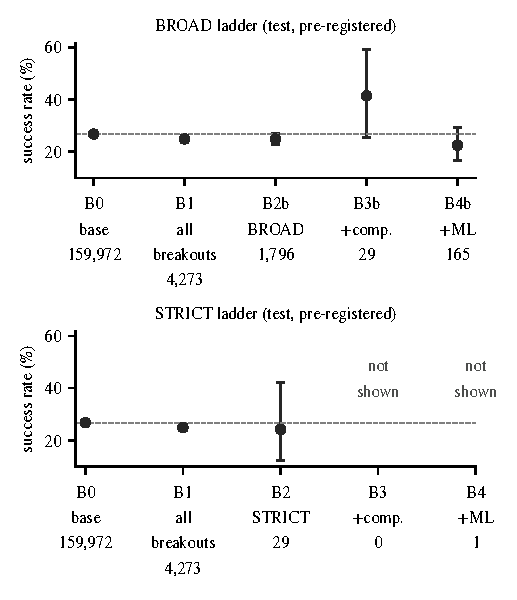
\includegraphics[width=\columnwidth]{figs/fig_ladder.pdf}
\caption{Pre-registered benchmark ladder during test period. Success rate for 10-days with Wilson 95\%
intervals (dashed line is total eligible stock-days base rate). Rungs with $<$2 events are identified but not
graphed.}
\label{fig:ladder}
\end{figure}

\subsection{Post-Hoc Analyses}
\emph{The tests in this subsection were all post-hoc analyses developed after opening the test set.}

\textbf{Cost break-even.} Average round-trip costs are 0.58\% (range 0.45--0.75\%). If the gross profits on
successful and unsuccessful events are +4.74\% and \ensuremath{-}1.85\%, respectively, then a success-rate change
$d$ only pays for 1 round trip if $d\ge 8.8$ pp. 95\% intervals for H1 (\ensuremath{-}4.4 to +4.3 [month block
\ensuremath{-}5.3 to +4.7]), H1 without the pilot (\ensuremath{-}2.8 to +8.1), and H2 (\ensuremath{-}6.8 to
+1.2) are within $\pm$8.8 pp. H2 without pilot-window (\ensuremath{-}5.65 pp [\ensuremath{-}10.6 to
\ensuremath{-}0.7]) hits the break-even point. For the composite top decile +7.0 pp [+0.6 to +13.4] above other
BROAD events (not including zero, but including the break-even point).

\textbf{Placebo.} The average placebo H1 effect is not 0, but +1.65 pp (SD 1.97), if you shuffle delivery
across stocks within each day 1,000 times. The delivery increase is a $z$-score to the trailing year per stock,
and since you shuffle within each day, the market-wide delivery level is constant, so there is a time-varying
market component in the placebo exposure. This isn't a clean null. The real \ensuremath{-}0.04 pp is at 20th
percentile (one-sided $p=0.795$, Fig.~\ref{fig:placebo}). There is no other stock-specific delivery
information, beyond this component. And the H1 effect in training/validation of +1.05 pp, which is higher than
all the 20 placebo draws in there, is not reproduced.

\begin{figure}[t]
\centering
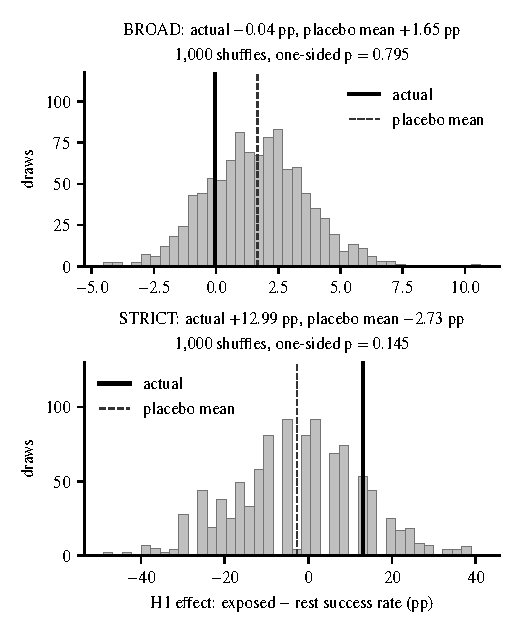
\includegraphics[width=\columnwidth]{figs/fig_placebo_hist.pdf}
\caption{Post-hoc placebo (test set). H1 effect for within-day shuffling of delivery among stocks. Real
effect shown. The shuffled distribution is non-zero-centered (see text).}
\label{fig:placebo}
\end{figure}

\textbf{Spec curve.} With varying barrier/horizon/threshold for delivery/event set (Fig.~\ref{fig:spec})
\cite{simonsohn2020}, 89\% of the 54 H1 specifications are in the predicted direction, 15 sig 5\% (0 in
opposite), 3 BH surviving. Median +2.36 pp, max 5.05 pp $<$ break-even. The preregistered specification
(\ensuremath{-}0.04 pp) is ranked 49 of 54. Higher thresholds, wider barriers lead to higher effects. H2: 3 sig
of 18, 0 surviving, median \ensuremath{-}2.24 pp. Specification frozen ranked 6. The specs are overlapping and
not independent.

\begin{figure*}[t]
\centering
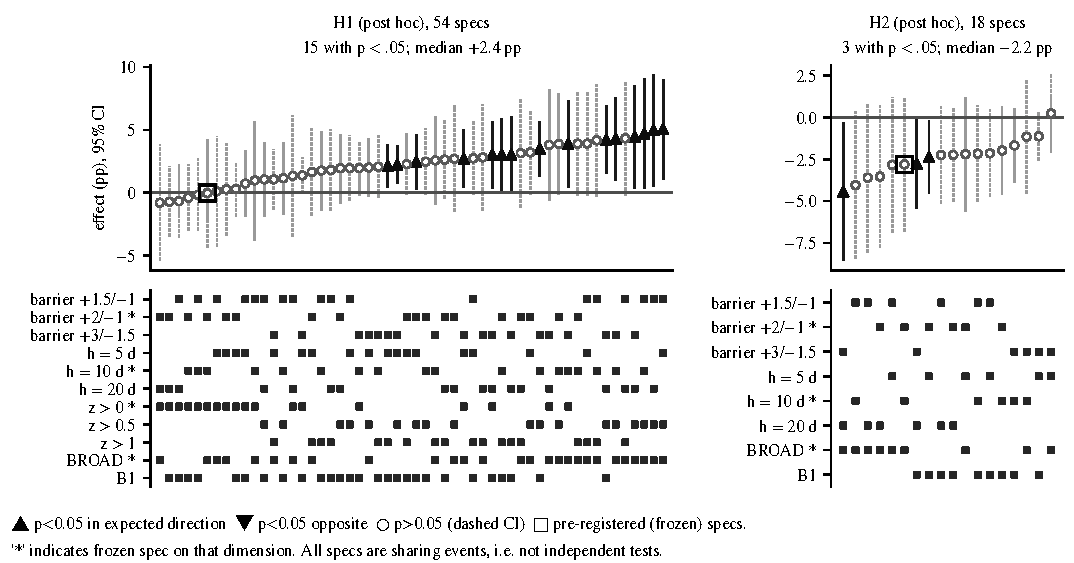
\includegraphics[width=\textwidth]{figs/fig_spec_curve.pdf}
\caption{Test set post-hoc specification curve. Top: Effect and 95\% confidence interval for each
specification. Bottom: Choices for specification. Square shows the pre-registered specification.}
\label{fig:spec}
\end{figure*}

\textbf{Bayes factors:} 17.88 (uniform prior \cite{kass1995}) and 8.41 (unit-normal log odds prior
\cite{gronau2021}) for H1 (BF$_{01}$), only 2.27--2.32 with sceptical priors; for H2: 7.65, 3.63 and
1.05--1.13. If no pilot window, H2 under sceptical beta prior: 0.23 (moderate evidence for difference). Only
strong evidence for null if wide priors \cite{leewagenmakers2013}.

\textbf{Cluster-robust model.} Two-way date $\times$ stock clustering \cite{cameron2011}. In
\eqref{eq:logit}, the test-set interaction is $\beta_3=+0.246$ [\ensuremath{-}0.130, +0.622] ($p=0.200$) for H1
and \ensuremath{-}0.186 ($p=0.142$) for H2. +0.185 ($p=0.043$) is a single post-hoc coefficient (not
multiplicity-adjusted) for the H2 model for delivery.

\textbf{Other tests.} H1 is \ensuremath{-}1.4 pp ($p=0.572$) without 5 sessions before 47 F\&O expiries.
None of 12 yearly H1 estimates are significant. Same day barrier ties are 0.12\% of breakouts loss. More often
breakouts are stopped out day 1 with bigger next day ranges (15.0\% vs 10.3\%).

\section{Discussion and Limitations}
PREREGISTERED: No effect on breakout success by delivery expansion, OI divergence or FII/DII regime, boosted
trees $<$ fixed composite, suggestive of drift in market-wide positioning features. NULL only informative on
large effects (Detectable effect $\sim$6.26 pp, not establishing $\pm$2 pp equiv., only strong null support from
Bayes factors with wide priors). Full test interval post hoc $<$ 8.8 pp cost break-even. 1 sub-sample doesn't
fit: without pilot window, H2 = \ensuremath{-}5.65 pp ($p=0.026$, $q=0.128$), 95\% interval touches
break-even. BF$_{01}$ (scept prior) 0.23 is moderate evidence for H2. This is a lead (post-hoc sub-sample
failing false discovery control). Pre-registered H1 spec among weakest (as in spec curve); maybe delivery
threshold stricter or wider barriers, post hoc effect a few pp (maybe information on move size but not
direction), mostly not multiply controlled, $<$ break-even.

\emph{Limitations:} Market-wide positions for participants only. Futures positions may be hedges.
``Client'' class includes both retail and wealthy. Too few STRICT events for inference. Data covers T+1
settlement (2023) and F\&O reforms (2024--2025). Full dataset preparation done prior to registration (with
revealed counts/base rates in test set), our pilot partially overlapped test period. Many post-hoc analyses.
Choices made post-knowledge of result.

\section{Conclusion and Future Work}
We study hypothesis testing on a NSE panel free from survivorship, where test set is only opened once and
hypothesis is pre-registered. The results show no evidence supporting the popular notion that delivery \&
futures positioning footprints can tell you about breakout success. There is no strategy that outperforms
Nifty~500, after costs. Though we do not completely rule out smaller effect, these effect sizes are below
Indian cost requirements on the full test set. The following four leads require pre-registered tests with
post-October-2026 data: (1) is FII price follower in stock futures? (2) Does FII positioning in index futures
lead index returns? (3) Stricter delivery threshold for breakout size prediction? (4) does price up OI down
divergence (H2) predict breakout failure. (it may according to post-hoc subset except pilot window). Also, we
intend to build a market-level regime transition model based on participant positioning to predict volatility
regimes. This will be pre-registered and will only be tested on post October 2026 data. This is not investment
advice.

\section*{Data and Code Availability}
Input files are publicly available NSE end-of-day files which are re-downloaded by the pipeline. The authors
can provide code and configuration, locked and post-hoc results, sources for each table/figure/number
(generators), and SHA-256 checksums for locked files upon request.

\FloatBarrier
\begin{thebibliography}{10}
\providecommand{\url}[1]{#1}
\csname url@samestyle\endcsname
\providecommand{\newblock}{\relax}
\providecommand{\bibinfo}[2]{#2}
\providecommand{\BIBentrySTDinterwordspacing}{\spaceskip=0pt\relax}
\providecommand{\BIBentryALTinterwordstretchfactor}{4}
\providecommand{\BIBentryALTinterwordspacing}{\spaceskip=\fontdimen2\font plus
\BIBentryALTinterwordstretchfactor\fontdimen3\font minus
  \fontdimen4\font\relax}
\providecommand{\BIBforeignlanguage}[2]{{%
\expandafter\ifx\csname l@#1\endcsname\relax
\typeout{** WARNING: IEEEtran.bst: No hyphenation pattern has been}%
\typeout{** loaded for the language `#1'. Using the pattern for}%
\typeout{** the default language instead.}%
\else
\language=\csname l@#1\endcsname
\fi
#2}}
\providecommand{\BIBdecl}{\relax}\BIBdecl

\bibitem{samantaray2026}
S.~P. Samantaray, S.~Mohapatra, and M.~Mishra, ``A wavelet-decomposed
  {$\Delta$}-band with constricted {PSO}-tuned light gradient boosting machine for {Indian} stock market
  prediction with cross-country market influence,'' \emph{IEEE Access}, vol.~14, pp. 87\,746--87\,773, 2026,
  doi: \url{10.1109/ACCESS.2026.3700317}.

\bibitem{singh2025}
P.~Singh, M.~Jha, and H.~Patel, ``Wavelet-enhanced deep learning ensemble for accurate
  stock market forecasting: A case study of {Nifty} 50 index,'' \emph{IEEE Access}, vol.~13, pp.
  87\,036--87\,047, 2025, doi: \url{10.1109/ACCESS.2025.3568634}.

\bibitem{kumar2025}
C.~R. Kumar and S.~Manikandan, ``{SEMP-TA}: A novel stock market prediction approach
  based on stacking ensemble machine learning for effective trend analysis,'' \emph{IEEE Access}, vol.~13, pp.
  117\,479--117\,490, 2025, doi: \url{10.1109/ACCESS.2025.3586233}.

\bibitem{rajagopal2026}
S.~Rajagopal, H.~Natraj, M.~Pavani, R.~Kumar, and R.~R. Roy, ``Automated alpha factor
  discovery using machine learning, deep learning, and explainable {AI} for transparent trading strategies,''
  \emph{IEEE Access}, vol.~14, pp. 116\,342--116\,358, 2026, doi: \url{10.1109/ACCESS.2026.3716293}.

\bibitem{easley1996}
D.~Easley, N.~M. Kiefer, M.~O'Hara, and J.~B. Paperman, ``Liquidity,
  information, and infrequently traded stocks,'' \emph{J. Finance}, vol.~51,
  no.~4, pp. 1405--1436, 1996, doi: \url{10.1111/j.1540-6261.1996.tb04074.x}.

\bibitem{easley2012}
D.~Easley, M.~M. L{\'o}pez~de Prado, and M.~O'Hara, ``Flow toxicity and
  liquidity in a high-frequency world,'' \emph{Rev. Financial Stud.}, vol.~25,
  no.~5, pp. 1457--1493, 2012, doi: \url{10.1093/rfs/hhs053}.

\bibitem{kyle1985}
A.~S. Kyle, ``Continuous auctions and insider trading,'' \emph{Econometrica},
  vol.~53, no.~6, pp. 1315--1335, 1985, doi: \url{10.2307/1913210}.

\bibitem{glosten1985}
L.~R. Glosten and P.~R. Milgrom, ``Bid, ask and transaction prices in a
  specialist market with heterogeneously informed traders,'' \emph{J. Financial
  Econ.}, vol.~14, no.~1, pp. 71--100, 1985, doi:
  \url{10.1016/0304-405X(85)90044-3}.

\bibitem{harvey2016}
C.~R. Harvey, Y.~Liu, and H.~Zhu, ``{\ldots}and the cross-section of expected
  returns,'' \emph{Rev. Financial Stud.}, vol.~29, no.~1, pp. 5--68, 2016, doi:
  \url{10.1093/rfs/hhv059}.

\bibitem{bailey2014pseudo}
D.~H. Bailey, J.~M. Borwein, M.~L{\'o}pez~de Prado, and Q.~J. Zhu,
  ``Pseudo-mathematics and financial charlatanism: The effects of backtest
  overfitting on out-of-sample performance,'' \emph{Notices Amer. Math. Soc.},
  vol.~61, no.~5, pp. 458--471, 2014, doi: \url{10.1090/noti1105}.

\bibitem{nosek2018}
B.~A. Nosek, C.~R. Ebersole, A.~C. DeHaven, and D.~T. Mellor, ``The
  preregistration revolution,'' \emph{Proc. Nat. Acad. Sci. USA}, vol. 115,
  no.~11, pp. 2600--2606, 2018, doi: \url{10.1073/pnas.1708274114}.

\bibitem{chen2016}
T.~Chen and C.~Guestrin, ``{XGBoost}: A scalable tree boosting system,'' in
  \emph{Proc. 22nd ACM SIGKDD Int. Conf. Knowl. Discov. Data Mining}, 2016, pp.
  785--794, doi: \url{10.1145/2939672.2939785}.

\bibitem{thapa2026}
C.~Thapa, B.~Neupane, C.~Shrestha, and N.~P. Bhattarai, ``Policy information
  uncertainty and foreign institutional investors trading behavior: Evidence
  from {India},'' \emph{Rev. Quant. Finance Account.}, vol.~67, pp. 45--79,
  2026, doi: \url{10.1007/s11156-025-01448-8}.

\bibitem{lu2024}
X.~Lu, J.~Poon, and M.~Khushi, ``Bridging the gap between machine and human in
  stock prediction: Addressing heterogeneity in stock market,'' \emph{IEEE
  Access}, vol.~12, pp. 186\,171--186\,185, 2024, doi:
  \url{10.1109/ACCESS.2024.3511613}.

\bibitem{fieberg2023}
C.~Fieberg, D.~Metko, T.~Poddig, and T.~Loy, ``Machine learning techniques for
  cross-sectional equity returns' prediction,'' \emph{OR Spectr.}, vol.~45,
  no.~1, pp. 289--323, 2023, doi: \url{10.1007/s00291-022-00693-w}.

\bibitem{azevedo2023}
V.~Azevedo and C.~Hoegner, ``Enhancing stock market anomalies with machine
  learning,'' \emph{Rev. Quant. Finance Account.}, vol.~60, no.~1, pp.
  195--230, 2023, doi: \url{10.1007/s11156-022-01099-z}.

\bibitem{farimani2024}
S.~A. Farimani, M.~V. Jahan, and A.~M. Fard, ``An adaptive multimodal learning
  model for financial market price prediction,'' \emph{IEEE Access}, vol.~12,
  pp. 121\,846--121\,863, 2024, doi: \url{10.1109/ACCESS.2024.3441029}.

\bibitem{lundberg2020}
S.~M. Lundberg, G.~Erion, H.~Chen, A.~DeGrave, J.~M. Prutkin, B.~Nair, R.~Katz,
  J.~Himmelfarb, N.~Bansal, and S.-I. Lee, ``From local explanations to global
  understanding with explainable {AI} for trees,'' \emph{Nature Mach. Intell.},
  vol.~2, no.~1, pp. 56--67, 2020, doi: \url{10.1038/s42256-019-0138-9}.

\bibitem{cerneviciene2024}
J.~{\v{C}}ernevi{\v{c}}ien{\.{e}} and A.~Kaba{\v{s}}inskas, ``Explainable
  artificial intelligence ({XAI}) in finance: A systematic literature review,''
  \emph{Artif. Intell. Rev.}, vol.~57, Art. no.~216, 2024, doi:
  \url{10.1007/s10462-024-10854-8}.

\bibitem{martins2024}
T.~Martins, A.~M. de~Almeida, E.~Cardoso, and L.~Nunes, ``Explainable
  artificial intelligence ({XAI}): A systematic literature review on taxonomies
  and applications in finance,'' \emph{IEEE Access}, vol.~12, pp. 618--629,
  2024, doi: \url{10.1109/ACCESS.2023.3347028}.

\bibitem{yeo2025}
W.~J. Yeo, W.~Van Der~Heever, R.~Mao, E.~Cambria, R.~Satapathy, and
  G.~Mengaldo, ``A comprehensive review on financial explainable {AI},''
  \emph{Artif. Intell. Rev.}, vol.~58, no.~6, Art. no.~189, 2025, doi:
  \url{10.1007/s10462-024-11077-7}.

\bibitem{bailey2014dsr}
D.~H. Bailey and M.~L{\'o}pez~de Prado, ``The deflated {Sharpe} ratio:
  Correcting for selection bias, backtest overfitting, and non-normality,''
  \emph{J. Portfolio Manage.}, vol.~40, no.~5, pp. 94--107, 2014, doi:
  \url{10.3905/jpm.2014.40.5.094}.

\bibitem{benjamini1995}
Y.~Benjamini and Y.~Hochberg, ``Controlling the false discovery rate: A
  practical and powerful approach to multiple testing,'' \emph{J. Roy. Statist.
  Soc. Ser. B (Methodol.)}, vol.~57, no.~1, pp. 289--300, 1995, doi:
  \url{10.1111/j.2517-6161.1995.tb02031.x}.

\bibitem{hansen2005}
P.~R. Hansen, ``A test for superior predictive ability,'' \emph{J. Bus. Econ.
  Statist.}, vol.~23, no.~4, pp. 365--380, 2005, doi:
  \url{10.1198/073500105000000063}.

\bibitem{white2000}
H.~White, ``A reality check for data snooping,'' \emph{Econometrica}, vol.~68,
  no.~5, pp. 1097--1126, 2000, doi: \url{10.1111/1468-0262.00152}.

\bibitem{minervini2013}
M.~Minervini, \emph{Trade Like a Stock Market Wizard}.\hskip 1em plus 0.5em
  minus 0.4em\relax New York, NY, USA: McGraw-Hill, 2013.

\bibitem{lopezdeprado2018}
M.~L{\'o}pez~de Prado, \emph{Advances in Financial Machine Learning}.\hskip 1em
  plus 0.5em minus 0.4em\relax Hoboken, NJ, USA: Wiley, 2018.

\bibitem{delong1988}
E.~R. DeLong, D.~M. DeLong, and D.~L. Clarke-Pearson, ``Comparing the areas
  under two or more correlated receiver operating characteristic curves: A
  nonparametric approach,'' \emph{Biometrics}, vol.~44, no.~3, pp. 837--845,
  1988, doi: \url{10.2307/2531595}.

\bibitem{brier1950}
G.~W. Brier, ``Verification of forecasts expressed in terms of probability,''
  \emph{Monthly Weather Rev.}, vol.~78, no.~1, pp. 1--3, 1950, doi:
  \url{10.1175/1520-0493(1950)078<0001:VOFEIT>2.0.CO;2}.

\bibitem{lakens2017}
D.~Lakens, ``Equivalence tests: A practical primer for $t$ tests, correlations,
  and meta-analyses,'' \emph{Social Psychol. Personality Sci.}, vol.~8, no.~4,
  pp. 355--362, 2017, doi: \url{10.1177/1948550617697177}.

\bibitem{simonsohn2020}
U.~Simonsohn, J.~P. Simmons, and L.~D. Nelson, ``Specification curve
  analysis,'' \emph{Nature Human Behav.}, vol.~4, no.~11, pp. 1208--1214, 2020,
  doi: \url{10.1038/s41562-020-0912-z}.

\bibitem{kass1995}
R.~E. Kass and A.~E. Raftery, ``Bayes factors,'' \emph{J. Amer. Statist.
  Assoc.}, vol.~90, no. 430, pp. 773--795, 1995, doi:
  \url{10.1080/01621459.1995.10476572}.

\bibitem{gronau2021}
Q.~F. Gronau, A.~Raj K.~N., and E.-J. Wagenmakers, ``Informed {Bayesian}
  inference for the {A/B} test,'' \emph{J. Statist. Softw.}, vol. 100, no.~17,
  2021, doi: \url{10.18637/jss.v100.i17}.

\bibitem{leewagenmakers2013}
M.~D. Lee and E.-J. Wagenmakers, \emph{Bayesian Cognitive Modeling: A Practical
  Course}.\hskip 1em plus 0.5em minus 0.4em\relax Cambridge, U.K.: Cambridge
  Univ. Press, 2013.

\bibitem{cameron2011}
A.~C. Cameron, J.~B. Gelbach, and D.~L. Miller, ``Robust inference with
  multiway clustering,'' \emph{J. Bus. Econ. Statist.}, vol.~29, no.~2, pp.
  238--249, 2011, doi: \url{10.1198/jbes.2010.07136}.

\end{thebibliography}

\end{document}